\chapter{Analiza i projekt systemu}

\section{Opis funkcjonalny systemu}
System zarządzania wizytami lekarskimi zapewnia funkcjonalność dla dwóch głównych typów użytkowników: \textbf{sekretariatu} oraz \textbf{pacjenta}. Każdy z użytkowników ma dostęp do dedykowanego panelu, zawierającego odpowiednie opcje i możliwości:

\begin{itemize}
  \item \textbf{Sekretariat:}
  \begin{itemize}
    \item przeglądanie, dodawanie, edytowanie i usuwanie danych pacjentów,
    \item zarządzanie wizytami: aktualizacja statusu, dodawanie notatek lekarskich,
    \item przeglądanie oraz zarządzanie lekarzami.
  \end{itemize}

  \item \textbf{Pacjent:}
  \begin{itemize}
    \item przeglądanie danych osobowych,
    \item przeglądanie historii wizyt wraz z notatkami od lekarza,
    \item rezerwacja nowej wizyty, wybierając lekarza i termin.
  \end{itemize}
\end{itemize}

\section{Diagram koncepcyjny bazy danych}
\begin{figure}[H]
\centering
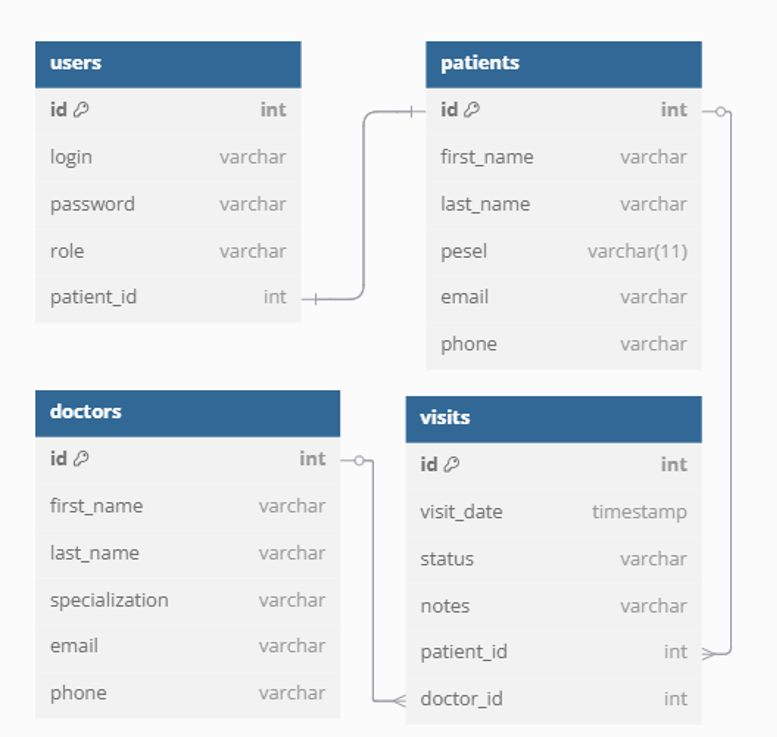
\includegraphics[width=0.85\textwidth]{figures/Diagram_bazy_danych.png}
\caption{Diagram koncepcyjny bazy danych}
\end{figure}

\section{Diagram klas (dziedziczenie)}
\begin{figure}[H]
\centering
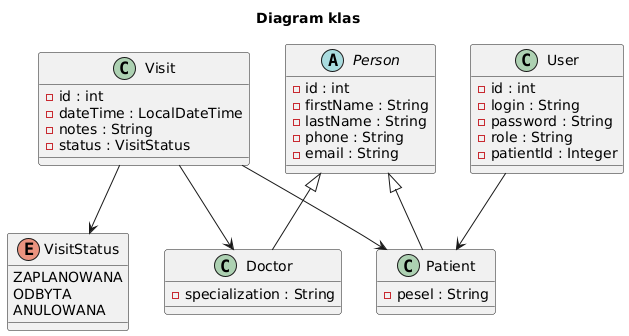
\includegraphics[width=0.85\textwidth]{figures/DiagramKlas.png}
\caption{Diagram klas przedstawiający hierarchię dziedziczenia}
\end{figure}

\section{Opis struktur danych}
System opiera się na czterech głównych encjach:
\begin{itemize}
  \item \textbf{Pacjent} -- dane identyfikacyjne (imię, nazwisko, PESEL, email, telefon),
  \item \textbf{Lekarz} -- imię, nazwisko, email, telefon, specjalizacja,
  \item \textbf{Wizyta} -- powiązanie lekarza z pacjentem, termin, status, notatka,
  \item \textbf{Użytkownik} -- login, hasło, rola (sekretarz lub pacjent), powiązanie z pacjentem (jeśli dotyczy).
\end{itemize}
